\chapter{Algorithms}

% introduction
In order to test if the proposed exoskeleton can aid in the training of the robots, a simulated environment with a task has been created in which a UR5 robot arm will have to pick-and-place virtual balls of varying stiffness into appropriate boxes. This task will be performed using three different methods: a classical approach, where the robot trajectory is generated from points; a reinforcement learning approach, where the robot aims to perform the task by trial and error while learning from past mistakes and optimizing a reward function; and lastly, inverse reinforcement learning, where the reward function is learned from human demonstration instead of being shaped by the machine learning engineer.

% import sections
\section{Background}

In this section we will recall how the...


\section{Task Description}

A custom simulated environment has been created in order to test the algorithms and the exoskeleton. The simulated environment consists of UR5 robot equiped with robotiq 140 gripper, placed on a table Fig. \ref{fig:environment_setup}. The robot is initialized with the home pose of $\mathbf{q}_0 = \begin{bmatrix} -1.57 & -1.55 & 1.34 & -1.37 & -1.57 & 0 \end{bmatrix}^T$ at coordinates $(x, y, z) = (0, 0, 1)$. The position of the ball is initialized randomly by sampling from an uniform distribution Eq. \ref{eq:ball_init}.

\begin{align}
  \mathbf{p}_{\text{ball}} &\sim \text{Uniform}(\mathbf{p}_{\min}, \mathbf{p}_{\max}) \label{eq:ball_init} \\
  \mathbf{p}_{\min} &= \begin{bmatrix} -0.38 \\ -0.55 \\ 1 + r_{\text{ball}} \end{bmatrix}, \quad
  \mathbf{p}_{\max} = \begin{bmatrix} 0.38 \\ -0.38 \\ 1 + r_{\text{ball}} \end{bmatrix}
\end{align}

\begin{figure}[ht]
  \centering
  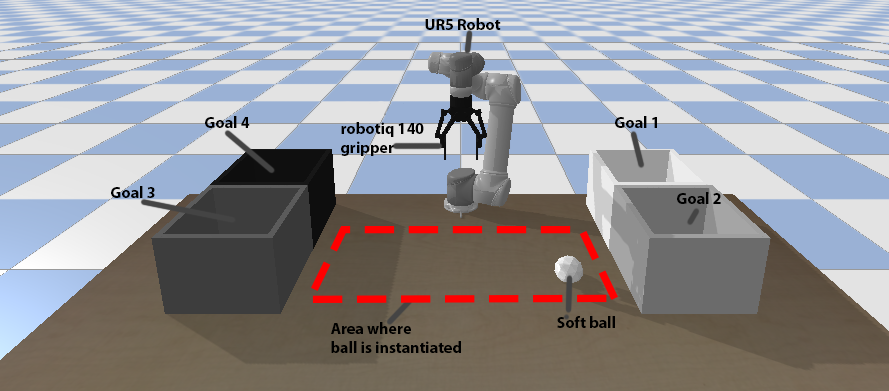
\includegraphics[width=1\textwidth]{chapters/algorithms/images/Environment_setup.png}
  \caption{Environment setup.}
  \label{fig:environment_setup}
\end{figure}

\noindent
During the initialization, the soft ball is assigned one of the four possible types Tab. \ref{tab:ball_classes}, the stiffness of each type varies based on the Young's Modulus. There are four boxes: $\mathbf{p}_{\text{goal},1} = (0.70, -0.16, 1), \mathbf{p}_{\text{goal},2} = (0.70, -0.50, 1), \mathbf{p}_{\text{goal},3} = (-0.70, -0.50, 1), \mathbf{p}_{\text{goal},4} = (-0.70, -0.16, 1)$. The boxes dimensions are 30x30x25cm and the walls are 2cm thick. The goal of the robot is to pick the ball and sort it according to it's type to the appropriate box. 

\begin{table}[ht]
  \centering
  \setlength{\tabcolsep}{6pt}
  \setlength{\abovecaptionskip}{6pt}
  \begin{tabular}{@{}cccc@{}}
      \toprule
      \textbf{Ball Type} & \textbf{Young's Modulus [min, max]} & \textbf{Density $(kg/m^3)$} & \textbf{Poisson's ratio} \\ 
      \midrule
      1 & [900, 1100] & 400 & 0.4 \\ 
      2 & [1400, 1600] & 400 & 0.4 \\ 
      3 & [1900, 2100] & 400 & 0.4 \\ 
      4 & [2400, 2600] & 400 & 0.4 \\ 
      \bottomrule
  \end{tabular}
  \caption{Ball types and their respective properties.}
  \label{tab:ball_classes}
\end{table}
\section{Implementation}
The three algorithms: classical, reinforcement learning and inverse reinforcement learning have been implemented.

\subsection{Classical Algorithm}
A classical algorithm consists of the following steps: ball detection, trajectory generation and ball classification. Each of these will be discussed in greater detail.

\subsubsection{Ball Detection}
The simulator provides the precise position and orientation of the ball in world coordinates, but in real use case this information would need to be acquired. In order to immitate the real world, the ball position will be found with the use of camera. One way robots can detect objects in the physical world is to extract depth information from the environment with the use of two or more regular cameras and perform triangulation. Similar to biological process of stereopsis. Depth cameras such as Intel Realsense make this an easy to implement solution. There are also different methods such as structured light or time of flight. There will be no need to manually perform triangulation in PyBullet as it has getCameraImage function which can return a depth image.
The PyBullet uses OpenGL, when the scene is rendered, the OpenGL stores depth values as a part of rendering pipeline. It is important to understand the camera model and the order of transformations used to obtain the depth buffer in order to inverse this process to obtain the point cloud of the scene.

\bigskip \noindent
The first transformation is performed by the view matrix. This matrix is used to transform the vertixes of the scene in the world space to the scene in the camera's view space, as it is desired to render the scene from the view of the camera. In other words, a view matrix is such a matrix that will transfrom the camera object to the center of origin in the world coordinates. Since the PyBullet uses right-hand coordinate system, the transformed camera's object Z-axis must be inverted, it must look down instead of up.

\bigskip \noindent
The OpenGL uses look-at camera method. This method describes the camera by it's position in world coordinates (called eye-position, denoted as E), target point (the point the camera looks at, denoted as C) and up vector (usually $[0, 1, 0]$, denoted as U). The camera has following rotation and translation matrices defining it's position and orientation Eq. \ref{eq:cam_t_r}

\begin{align}
  R =
  \begin{bmatrix}
  R_x & U'_x & F_x & 0 \\
  R_y & U'_y & F_y & 0 \\
  R_z & U'_z & F_z & 0 \\
  0   & 0   & 0   & 1
  \end{bmatrix}, \quad
  T =
  \begin{bmatrix}
  1 & 0 & 0 & E_x \\
  0 & 1 & 0 & E_y \\
  0 & 0 & 1 & E_z \\
  0   & 0   & 0   & 1
  \end{bmatrix}
  \label{eq:cam_t_r}
\end{align}

\noindent
The right, up and forward basis vectors can be calculated from look-at camera parameters \cite{3dgep_view_matrix}

\begin{align}
  F &= \frac{C - E}{\|C - E\|}, \\
  R &= \frac{F \times U}{\|F \times U\|}, \\
  U' &= R \times Z
\end{align}

\noindent
The view matrix is a matrix that would align the camera to the origin of the world (with negative z axis for right hand coordinate system)

\begin{equation}
  \begin{aligned}
    M_{view}TR &=   \begin{bmatrix}
      1 & 0 & 0 & 0 \\
      0 & 1 & 0 & 0 \\
      0 & 0 & -1 & 0 \\
      0 & 0 & 0 & 1
      \end{bmatrix}  
      \Rightarrow \\ 
    M_{view} &= \begin{bmatrix}
        1 & 0 & 0 & 0 \\
        0 & 1 & 0 & 0 \\
        0 & 0 & -1 & 0 \\
        0 & 0 & 0 & 1
        \end{bmatrix} R^{-1}T^{-1} 
        \Rightarrow \\ 
    M_{view} &= \begin{bmatrix}
          1 & 0 & 0 & 0 \\
          0 & 1 & 0 & 0 \\
          0 & 0 & -1 & 0 \\
          0 & 0 & 0 & 1
          \end{bmatrix} R^{T}T^{-1} 
          \Rightarrow \\ 
    M_{view} &= \begin{bmatrix}
            1 & 0 & 0 & 0 \\
            0 & 1 & 0 & 0 \\
            0 & 0 & -1 & 0 \\
            0 & 0 & 0 & 1
            \end{bmatrix}  
            \begin{bmatrix}
              R_x & R_y & R_z & 0 \\
              U'_x & U'_y & U'_z & 0 \\
              F_x & F_y & F_z & 0 \\
              0   & 0   & 0   & 1
              \end{bmatrix}  
            \begin{bmatrix}
                1 & 0 & 0 & -E_x \\
                0 & 1 & 0 & -E_y \\
                0 & 0 & 1 & -E_z \\
                0   & 0   & 0   & 1
                \end{bmatrix}  
                \Rightarrow \\ 
    M_{view} &= \begin{bmatrix}
                  R_x & R_y & R_z & -(R \cdot E) \\
                  U'_x & U'_y & U'_z & -(U' \cdot E) \\
                  -F_x & -F_y & -F_z & (F \cdot E) \\
                  0   & 0   & 0   & 1
                  \end{bmatrix}
  \end{aligned}
  \end{equation}

\noindent
The second transformation is performed by the projection matrix \cite{songho_opengl_transform} Eq. \ref{eq:M_proj}, where r,l,t,b is the distance from the center if the near place, to the right, left, top and bottom bounds respectively. The n and f are near and far plane distance. Thr projection matrix projects points from camera's frustum to Normalized Device Coordinates (NDC) Fig \ref{fig:projection_matrix}. The clip space is an intermediate step in this process, where vertexes outside the clip space are clipped and discarded before the homogeneous division is performed. 

\begin{figure}[ht]
  \centering
  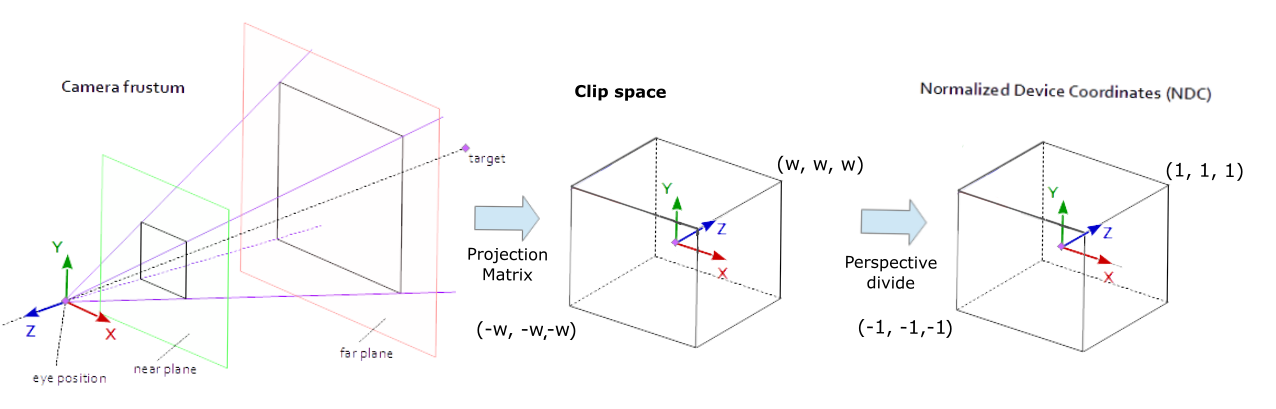
\includegraphics[width=1\textwidth]{chapters/algorithms/images/projection_matrix.png}
  \caption{Projection matrix}
  \label{fig:projection_matrix}
\end{figure}

\begin{equation}
  M_{proj} = \begin{bmatrix}
    \frac{2n}{r-l} & 0 & \frac{r+l}{r-l} & 0 \\
    0 & \frac{2n}{t-b} & \frac{t+b}{t-b} & 0 \\
    0 & 0 & \frac{-(f+n)}{f-n} & \frac{-2fn}{f-n} \\
    0 & 0 & -1 & 0
    \end{bmatrix}
  \label{eq:M_proj}
\end{equation}

\noindent
Now, with this knowledge it is possible to reverse this process to obtain a scene pointcloud in world coordinates from the depth image. The depth image pixels, ranges from 0 (near plane) to 1 (far plane). The first step is to convert the depth image to NDC space.

\begin{algorithm}[H]
  \caption{Converting depth image to homogeneous NDC space}
  \begin{algorithmic}[1]
  \State \textbf{Input:} depth\_img
  \State \textbf{Output:} NDC
  \For{$h = 0$ \textbf{to} depth\_img.height}
      \For{$w = 0$ \textbf{to} depth\_img.width}
          \State $x \gets \frac{2w - \text{depth\_img.width}}{\text{depth\_img.width}}$
          \State $y \gets -\frac{2h - \text{depth\_img.height}}{\text{depth\_img.height}}$
          \State $z \gets 2 \times \text{depth\_img}[h, w] - 1$
          \State NDC.append([x, y, z, 1])
      \EndFor
  \EndFor
  \end{algorithmic}
\end{algorithm}

\noindent
Now the NDC space can be converted to a point cloud by pre-multiplying it with the transformation matrix $\text{M}_{\text{NDC\_to\_World}}$ (Eq. \ref{eq:ndc_to_world}) and performing homogeneous division.

\begin{equation}
\text{M}_{\text{NDC\_to\_World}} = \left( \text{M}_{\text{proj}} \cdot \text{M}_{\text{view}} \right)^{-1}
\label{eq:ndc_to_world}
\end{equation}

\noindent
The point cloud of a scene, when a camera is placed a meter above the table and the robot arm is moved out of view can be seen in Fig. \ref{fig:pointcloud}.

\begin{figure}[h!]
    \centering
    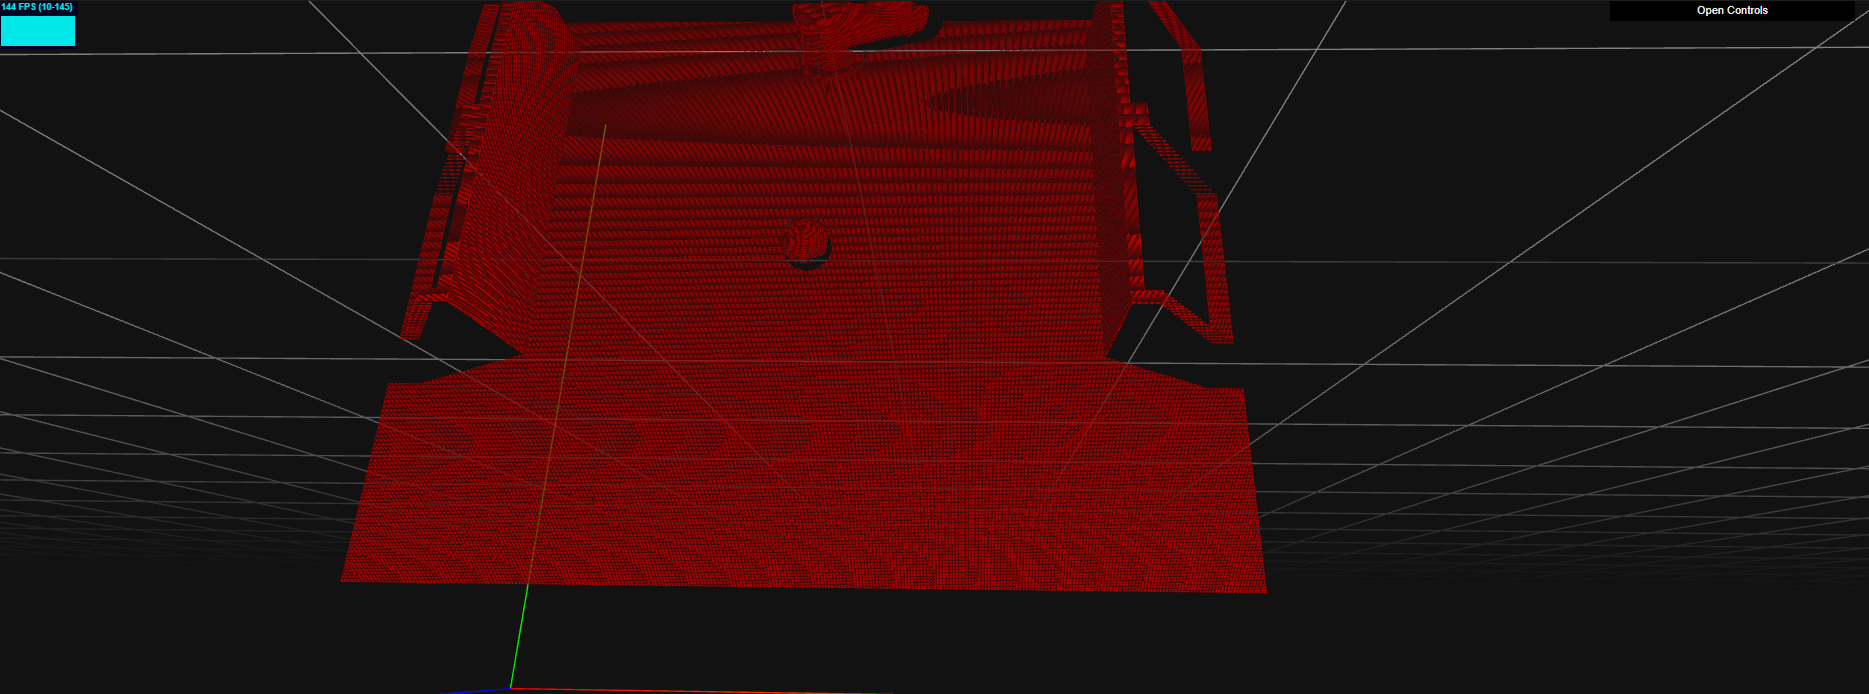
\includegraphics[width=\textwidth]{chapters/algorithms/images/Pointcloud.png}
    \caption{Scene point cloud.}
    \label{fig:pointcloud}
\end{figure}

The point cloud is further processed by cropping it to the working area only. This is a common method for speeding up localization. Then global alignment is performed by extracting features for the scene and object, obtaining correspondences, and using RANSAC to randomly sample 3 correspondences, aligning the object with the correspondences, and counting inliers. After 200 iterations, the pose with the highest inlier count is returned. The iterative closest point algorithm is not performed as orientation does not matter for a spherical object.
\section{Conclusion}
Three different algorithms for the robot pick-and-place task have been tested. The classical algorithm is the most reliable. It also provides high control over the behavior. The issues with classification can be improved by retraining the NN with the suggestions that were mentioned in the previous section, and the issues with gripping can be improved by redesigning a gripper. The RL took a significant amount of time, and yet it is not able to complete the task. The control over the behavior is limited. The reward signal and hyperparameters need to be readjusted, and the model needs to be retrained. This is a lengthy and expensive process. The trajectory collection within VR with \nametwo was successful. The training took significantly less time, and the behavior is an improvement over the RL. The biggest issue with GAIL-IRL was the discriminator becoming strong early on, leading to premature convergence of the policy. These results show that manually programming the behavior can take less time and provide higher control over the behavior compared to the tested AI methods. Classical methods should be preferred in tasks where they can be implemented easily. 
